\documentclass{beamer}

\mode<presentation>
\usepackage{amsmath,amssymb,mathtools}
\usepackage{textcomp}
\usepackage{gensymb}
\usepackage{adjustbox}
\usepackage{subcaption}
\usepackage{enumitem}
\usepackage[utf8]{inputenc}
\usepackage{amssymb}
\usepackage{enumitem}
\setlist{nosep} % optional: removes vertical gaps
\setlist[enumerate]{label=\arabic*)} % custom numbering if you want

\usepackage{multicol}
\usepackage{listings}
\usepackage{url}
\usepackage{graphicx} % <-- needed for images
\def\UrlBreaks{\do\/\do-}

\usetheme{Boadilla}
\usecolortheme{lily}
\setbeamertemplate{footline}{
  \leavevmode%
  \hbox{%
  \begin{beamercolorbox}[wd=\paperwidth,ht=2ex,dp=1ex,right]{author in head/foot}%
    \insertframenumber{} / \inserttotalframenumber\hspace*{2ex}
  \end{beamercolorbox}}%
  \vskip0pt%
}
\setbeamertemplate{navigation symbols}{}

\lstset{
  frame=single,
  breaklines=true,
  columns=fullflexible,
  basicstyle=\ttfamily\tiny    % tiny font so code fits
}

\numberwithin{equation}{section}

% ---- your macros ----
\providecommand{\nCr}[2]{\,^{#1}{#2}}
\providecommand{\nPr}[2]{\,^{#1}P_{#2}}
\providecommand{\mbf}{\mathbf}
\providecommand{\pr}[1]{\ensuremath{\Pr\left(#1\right)}}
\providecommand{\qfunc}[1]{\ensuremath{Q\left(#1\right)}}
\providecommand{\sbrak}[1]{\ensuremath{{}\left[#1\right]}}
\providecommand{\lsbrak}[1]{\ensuremath{{}\left[#1\right.}}
\providecommand{\rsbrak}[1]{\ensuremath{\left.#1\right]}}
\providecommand{\brak}[1]{\ensuremath{\left(#1\right)}}
\providecommand{\lbrak}[1]{\ensuremath{\left(#1\right.}}
\providecommand{\rbrak}[1]{\ensuremath{\left.#1\right)}}
\providecommand{\cbrak}[1]{\ensuremath{\left\{#1\right\}}}
\providecommand{\lcbrak}[1]{\ensuremath{\left\{#1\right.}}
\providecommand{\rcbrak}[1]{\ensuremath{\left.#1\right\}}}
\theoremstyle{remark}


\providecommand{\abs}[1]{\left\vert#1\right\vert}
\providecommand{\res}[1]{\Res\displaylimits_{#1}}
\providecommand{\norm}[1]{\lVert#1\rVert}
\providecommand{\mtx}[1]{\mathbf{#1}}
\providecommand{\mean}[1]{E\left[ #1 \right]}
\providecommand{\fourier}{\overset{\mathcal{F}}{ \rightleftharpoons}}

\providecommand{\dec}[2]{\ensuremath{\overset{#1}{\underset{#2}{\gtrless}}}}

\usepackage{gvv}
% ---------------------

\title{Matgeo Presentation - Problem 5.2.56}
\author{EE25BTECH11054 - S.Harsha Vardhan}

\begin{document}

%---------------- Title Page ----------------
\begin{frame}
  \titlepage
\end{frame}

%---------------- Problem Statement ----------------
\begin{frame}{Problem Statement}
	Solve the following system of linear equations.
	\[
	\frac{5}{x-1} + \frac{1}{y-2} = 2 \quad
	\frac{6}{x-1} - \frac{3}{y-2} = 1
	\]
\end{frame}

%---------------- Solution ----------------
\begin{frame}{Solution: Substitution}
	Let 
	\begin{align}
		u = \frac{1}{x-1}, \quad v = \frac{1}{y-2}.
	\end{align}
	The given system becomes a linear system in terms of $u$ and $v$:
	\begin{align}
		5u + v &= 2 \\
		6u - 3v &= 1
	\end{align}
\end{frame}

\begin{frame}{Solution: Matrix Form}
	In matrix form, this is $\vec{A}\vec{x} = \vec{b}$, where:
	\begin{align}
		\myvec{5 & 1 \\ 6 & -3} \myvec{u \\ v} = \myvec{2 \\ 1}.
	\end{align}
	Let 
	\begin{align}
		\vec{A} = \myvec{5 & 1 \\ 6 & -3}, \quad \vec{b} = \myvec{2 \\ 1}.
	\end{align}
	We can solve this using Gauss-Jordan elimination on the augmented matrix $\myvec{\vec{A}|\vec{b}}$.
\end{frame}

\begin{frame}{Solution: Gauss-Jordan Elimination}
	\begin{align}
		\augvec{2}{1}{5 & 1 & 2 \\ 6 & -3 & 1}
		&\xrightarrow{R_1 \rightarrow \frac{1}{5}R_1}
		\augvec{2}{1}{1 & \frac{1}{5} & \frac{2}{5} \\ 6 & -3 & 1}
		\xrightarrow{R_2 \rightarrow R_2 - 6R_1}
		\augvec{2}{1}{1 & \frac{1}{5} & \frac{2}{5} \\ 0 & -\frac{21}{5} & -\frac{7}{5}} 
	\end{align}
\end{frame}

\begin{frame}{Solution: Gauss-Jordan Elimination}
	\begin{align}
		\augvec{2}{1}{1 & \frac{1}{5} & \frac{2}{5} \\ 0 & -\frac{21}{5} & -\frac{7}{5}}
        &\xrightarrow{R_2 \rightarrow -\frac{5}{21}R_2}
		\augvec{2}{1}{1 & \frac{1}{5} & \frac{2}{5} \\ 0 & 1 & \frac{1}{3}} 
		\xrightarrow{R_1 \rightarrow R_1 - \frac{1}{5}R_2}
		\augvec{2}{1}{1 & 0 & \frac{1}{3} \\ 0 & 1 & \frac{1}{3}}
	\end{align}
\end{frame}

\begin{frame}{Solution: Back-Substitution}
From the reduced row echelon form, we have the solution for $u$ and $v$:
	\begin{align}
		\myvec{u \\ v} = \myvec{\frac{1}{3} \\ \frac{1}{3}}
	\end{align}
	Now, we back-substitute to find $x$ and $y$:
	\begin{align}
		u = \frac{1}{x-1} = \frac{1}{3} &\implies x - 1 = 3 \implies x = 4, \\
		v = \frac{1}{y-2} = \frac{1}{3} &\implies y - 2 = 3 \implies y = 5.
	\end{align}
\end{frame}

\begin{frame}{Solution: Final Answer}
Thus, the final solution is:
	\begin{align}
		\myvec{x \\ y} = \myvec{4 \\ 5}.
	\end{align}
\end{frame}

\begin{frame}{Plot}
    \begin{figure}[h]
    \centering
    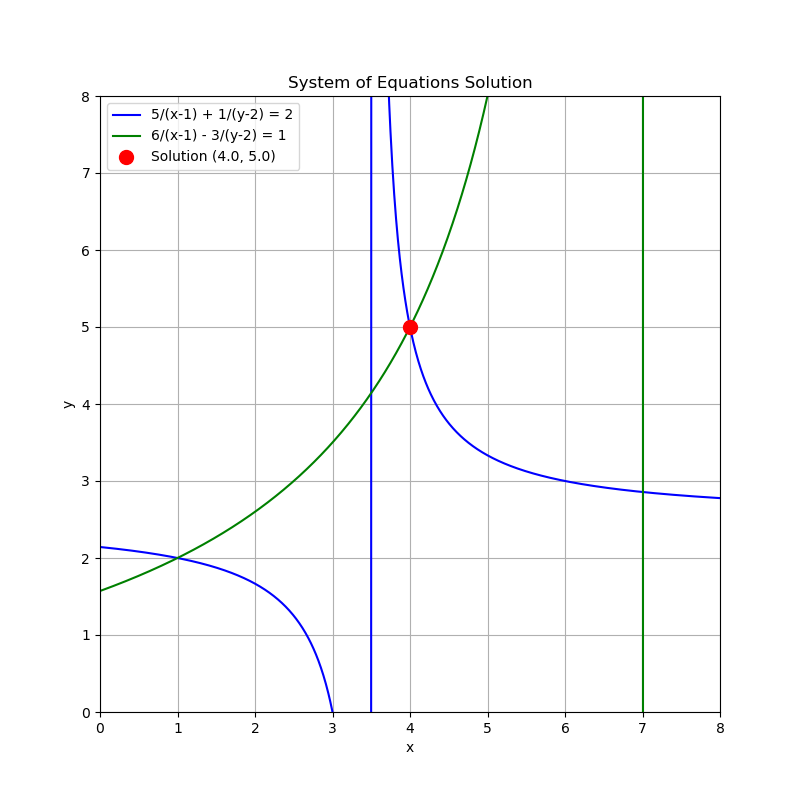
\includegraphics[width=0.6\columnwidth]{../figs/Figure_4.png}
    \caption*{}
    \label{fig:placeholder}
    \end{figure}
\end{frame}

\end{document}